%scb-term-paper.tex 
\documentclass[12pt]{article}
\usepackage{times}
\usepackage{amsmath,amssymb,latexsym}
\usepackage[round,sort]{natbib}
\usepackage{multirow,array}
\usepackage{fancyhdr}
\usepackage{lastpage}
\usepackage{graphicx}
\usepackage[bottom]{footmisc}
\graphicspath{ {scb-term-paper-images/} }
\usepackage[T1]{fontenc}
\usepackage{mathptmx}
\usepackage{tabu}
\usepackage{textcomp}
\usepackage{stata}
\usepackage{listings}
\usepackage[a4paper,margin=1.0in]{geometry}
\usepackage{multirow}
\usepackage{caption}
\usepackage{setspace}
\usepackage{verbatim}
\usepackage{pdflscape}
\usepackage{longtable}
\usepackage{hyperref}
\hypersetup{
    colorlinks=true,
    linkcolor=blue,
    filecolor=magenta,      
    urlcolor=cyan,
    citecolor=magenta,
}
\lstset{
basicstyle=\ttfamily,
columns=flexible,
breaklines=true
}
\newenvironment{hypothesis}{
  	\itshape
  	\leftskip=\parindent \rightskip=\parindent
  	\noindent\ignorespaces}
	
\setlength\parindent{0pt}
\pagestyle{fancy}
\fancyhf{}
\lhead{Strategy Content (B) Term Paper}
\rfoot{Page \thepage  \ of \pageref{LastPage}}
\rhead{Iyenggar}
\newcommand\question[2]{\vspace{1em}\hrule\vspace{1em}\textbf{#1}{ #2}\vspace{1em}\hrule\vspace{1em}}

\begin{document}
\title{\LARGE Heterogeneity in knowledge spillovers across regions:\\ \Large The effects of endogeneity,  complexity and IPR environment}
\author{Ashwin Iyenggar  (1521001) \\ ashwin.iyenggar15@iimb.ernet.in} 
\large

\maketitle
\thispagestyle{empty}

\begin{abstract}
\large \noindent I line up empirical evidence to demonstrate the heterogeneity in the geographical distribution of knowledge spillovers across various regions. I then explore  three potential mechanisms that may help explain this heterogeneity: endogenous aspects of the regions themselves, complexity of work, and the intellectual property rights environment. While the empirical results are yet inconclusive and incomplete, the current work extends prior work on geographic spillovers of knowledge by  integrating three alternative explanations.
\end{abstract}
{Keywords:} Knowledge Spillovers, Endogeniety, Complexity, IPR
\doublespacing
\section{Introduction}
There has been a long and illustrious scholarly tradition highlighting the agglomeration characteristics of economic regions, going back at least as far as \cite{Marshall1890}, whose original work was published in 1890. More recently, scholars over the last three decades have demonstrated the paper trail of these knowledge spillovers through the study of patent citations (e.g., \cite{Jaffe1993, Almeida1999}). This tradition of scholarship has further shaped our theoretical understanding of knowledge spillovers through mechanisms  the effects of inventor mobility (e.g., \cite{Almeida1999}), differential Intellectual Property Rights regime of locations (e.g., \cite{Zhao2006}) and of the role of international geography (e.g., \cite{Singh2007}).  The nature and extent of the geographical distribution of knowledge spillovers observed  in practice is so highly heterogenous across locations, firms and legal environments,  that the understanding of the causal mechanisms leading to knowledge spillovers continues to intrigue the best of scholars. While this is, in no way dismissive of  the enormous theoretical strides so far, the question is assumes greater significance in the environment surrounding the second machine age as some scholars have begun to highlight \citep{Mcafee2014} 
\\\\
Motivated by empirical evidence surrounding the heterogeneity in the nature of knowledge flows across the various regions, I intend to explore the three mechanisms ostensibly influencing knowledge spillovers. Complexity of patents invented as a potential mechanism influencing the extent of local knowledge spillovers. This approach is not yet another departure from the current theory on spillovers in management literature for the following reasons.  First, from a human capital perspective, it is valuable to understand the impact of MNCs that dominate much of the cutting- and bleeding-edge innovation in emerging markets on the development of the talent pool in the host country. Does a significant group of local inventors develop? Is this affected by the strength of the IPR regime in the host country? Second, a specific flavor of this question is the investigation of the spillover effects of the innovation process in emerging countries, or those known to have weaker IPR regimes. Specifically, do multinational firms that develop patentable technologies in emerging (or weaker IPR) countries create spillover effects in the host country talent pool? Or do the benefits remain localized to within multinational companies (MNCs) and their home country employees?  Finally, the wide disparity in the extent of knowledge spillovers across locations, across firms and across IPR regimes is intriguing to the researcher and calls attention toward a creative response.  a researcher to find the mechanisms that may lie behind such a phenomenon. Patents data allows us to ask these questions and to have them answered as has been in the tradition of \cite{Jaffe1993}.
\\\\
Complexity may be seen as either an attribute of usage, or as an attribute of invention. A patent that is used (cited) by several patents belonging to distinct and different patent technology classes maybe seen as modular by virtue of it being able to be plugged into multiple diverse applications. Alternatively a patent that is constructed with few dependencies may also be seen as being modular by virtue of its capacity to be developed standalone, or with minimal intervention from other modules. For the purposes of my study, I use a definition of Complexity that captures both the effects above. 
\\\\
Prior literature has looked at knowledge spillovers within geographic regions (e.g., \cite{Jaffe1993}) as well as across regions (e.g., \cite{Singh2007}). For the purposes of my study, I refer to local knowledge spillovers as those that occur within an adjacent geographical area. This is in keeping with my objective of trying to understand the local impact of inventing activity by multinationals in emerging nations. 
\\\\
This article therefore, attempts to answer the following questions. First, does the Complexity of patents developed across country borders differ from the Complexity of patents that are developed within a country? Second, does the Complexity of patents differ by the strength of the IPR regime of the inventor location? Finally, does the Complexity of patents affect the extent of local knowledge spillovers? 
\\\\
I am interested in understanding the spillover effects of patenting in emerging countries. Specifically, do multinational firms that develop patentable technologies in emerging countries end up creating spillover effects in the host country talent pool, or do the benefits remain localized to within MNCs. My focus in on human capital, and I wish to understand the impact of a allowing MNC's dominate the patenting process in emerging markets on the quality of the talent pool in the host country. Specifically, is there a significant group of local inventors who develop? Do they then move around to cross-pollinate to other firms? Or do domestic firms get completely left out. Does the talent pool demonstrate a clear MNC vs Domestic company division, i.e., to employees who have previously worked at MNCs move only to other MNCs, and those who had previously worked at Domestic Firms only continue to do so? I may try and understand this from patent data though this may be a large question to be asked for all roles. But the specific context of highly skilled, technologically intensive inventive roles are definitely interesting to look at.
\\\\
How do the patenting patterns of inventors whose first patent was co-invented with someone living abroad compare with that of inventors whose first patent was co-invented with someone living in the same location.

I am interested in understanding the impact of cross-national inventions on subsequent patenting career of inventors in weak IPR (or emerging) countries. Do they end up patenting more from the weak IPR country or do they eventually move to a strong IPR country. Do they develop more local inventors or do they patent more with international collaborators?

\cite{Zhao2006} argues that competing firms may have a lower ability to imitate when the value of technology is highly dependent on the proprietary firm\textquotesingle s internal resources. We contend that that assumption is weakened significantly if the knowledge of this technology is codified and published, and when published work on related technologies cite a common prior art. \cite{Zhao2006} herself cites \cite{Kogut1993} suggesting that difficult to codify knowledge lends itself to more efficient transfer within the firm. Drawing on \cite{Cohen2000}, we thereby conclude that firms would have a greater incentive to keep such highly dependent technology developed in weaker IPR countries secret, rather than make this knowledge public. While \cite{Zhao2006} highlights the strength of internal firm linkages in identifying and appropriating the knowledge generated in weak IPR location subsidiaries, she does not emphasize the importance of secrecy. Indeed, she uses patenting data from weaker IPR location offices to substantiate her hypothesis, which we believe actually weakens her argument for the strength of internal firm linkages.

\section{Motivation}
We take a set of locations across the world and calculate a normalized measure of their spillover distribution across regions. 
\begin{figure}[h]
\begin{centering}
  \includegraphics[width=\textwidth]{SameRegionSameAssigneeFlows}
  \caption{Local and Internal Flows by Region}
  \label{fig:SameRegionSameAssigneeFlows}
\end{centering}
\end{figure}

\begin{figure}[h]
\begin{centering}
  \includegraphics[width=\textwidth]{SameRegionDiffAssigneeFlows}
  \caption{Local and External Flows by Region}
  \label{fig:SameRegionDiffAssigneeFlows}
\end{centering}
\end{figure}


\begin{figure}[h]
\begin{centering}
  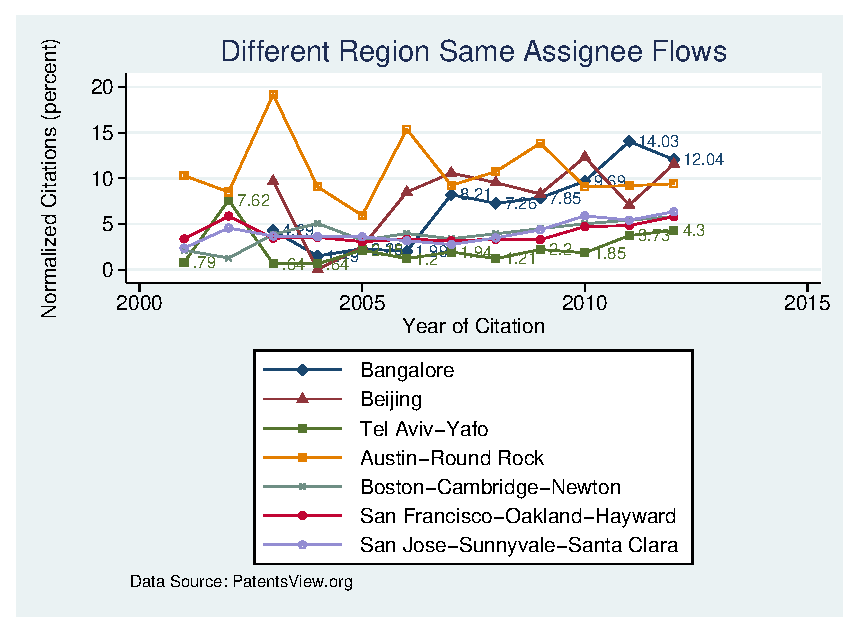
\includegraphics[width=\textwidth]{DiffRegionSameAssigneeFlows}
  \caption{Non-local and Internal Flows by Region}
  \label{fig:DiffRegionSameAssigneeFlows}
\end{centering}
\end{figure}

\begin{figure}[h]
\begin{centering}
  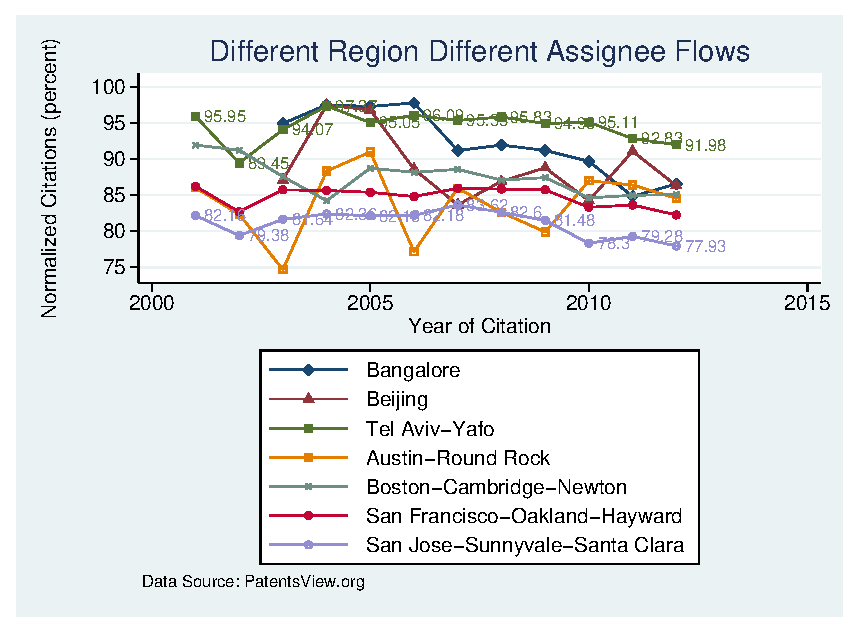
\includegraphics[width=\textwidth]{DiffRegionDiffAssigneeFlows}
  \caption{Non-local and External Flows by Region}
  \label{fig:DiffRegionDiffAssigneeFlows}
\end{centering}
\end{figure}


\section{Theory}
Lay the hypotheses here
\begin{hypothesis}{\\Hypothesis 1: I hope I can have something to go}\end{hypothesis}

\section{Research Design}
\subsection{Complexity}
I construct my measure of Complexity based interactions between the different patent sub-classes. Since each of the interactions between patent sub-classes may introduce a new interaction, I model interactions on a binomial function. Specifically, when \verb|subclass| represents the number of distinct patent sub-classes, I define  \verb|interaction(subclass)| as follows:

\begin{displaymath}
   interaction(subclass) = \left\{
     \begin{array}{lr}
       1 & : subclass \leq 2 \\
       \binom{subclass}{2} & : subclass > 2 \\
     \end{array}
   \right.
\end{displaymath} 

I would expect, from a user perspective that the more number of contexts in which the patent is valuable, the higher should be the Complexity. If \verb|Complexity| represents my measure of the Complexity of the patent, and \verb|usage contexts| represents the number of distinct contexts where the patent is found valuable, I should expect the following relationship to hold:
\begin{center}$ \verb|Complexity| \propto \frac{1}{usage \ contexts} $ \end{center}
Similarly, from an inventor perspective, the more the number of contexts that the patent is built on, the lower should be the Complexity. A patent that is developed without citing any other patents is an extreme case of highest Complexity, while one that requires to be built upon several \verb|source contexts| is properly understood as being less modular. The relationship between \verb|source contexts| and \verb|Complexity| is therefore an inverse one as depicted below.
\begin{center}$ \verb|Complexity| \propto source contexts $ \end{center} 

Using the principles above, I therefore develop the following definition of Complexity.
\begin{center}$ \verb|Complexity| = \frac{interaction(subclass_{\text{cited}})}{interaction(subclass_{\text{patent}})} $ \end{center}

By the definition above, a patent that cites no patents (and hence has $subclass_{\text{cited}} = 0$) but is itself assigned to 4 sub-classes (and hence has $subclass_{\text{patent}} = 4$) will have a raw Complexity score of $\frac{\binom{4}{2}}{1} = 6$. If the patent itself had been assigned onto to 2 sub-classes, the raw Complexity score would have been just 1. Therefore, the more the number of patent sub-classes a patent is assigned to, the higher its Complexity score (by a square term). A similar but inverse relationship would hold for sub-classes arising out of cited patents. Here, I take a set union of patent sub-classes assigned to each cited patent, and use that count to determine the value of the \verb|interaction| function.

\subsection{IPR Classification}
A review of the academic literature surrounding the construction of IPR indexes indicated that there were several, as was also evident in \cite{Zhao2006} constructing a composite measure for the purposes of her article. \cite{Lesser2010} provides an alternative, composite scoring system that includes the following components: protectable subject matter, membership in convention, enforcement, administration and duration of protection. I have therefore used the scores generated by \cite{Lesser2010} for the purposes of this study. The extensive table of IPR scores in presented in Table ~\ref{long}. The listing has several countries for which scores have not been provided. However none of the top patenting nations were among them, and I therefore chose to go along with this scale.

\subsection{Data Source}
I derive all patents data for this study from patentsview.org. The dataset considered is for all USPTO patents filed in the period 1976 to 2015. For the IPR Scores, I rely on the scores generated by \cite{Lesser2010}. For country definitions, I use the resources provided by \href{http://thematicmapping.org/downloads/world_borders.php}{Thematic Mapping}. To determine if spillovers are local, I use a composite data source as described in the following. For locations in the United States, it has been standard to use Metropolitan Statistical Areas (MSA) for analyses related to economic geography. Such standardized data is unavailable for non-US locations. Urban areas are a close substitute for  economic centers, and I therefore determine to use one such definition for non-US locations. My data source for MSA of US locations is \href{http://www.census.gov/geo/maps-data/data/cbf/cbf_msa.html}{the US census} and that for urban areas for world wide locations is \href{http://www.naturalearthdata.com/downloads/10m-cultural-vectors/}{Natural Earth Data}.
 
This automatically raises conflicting definitions for locations in the United States. So that the MSA definitions take precedence, I eliminated all data pertaining to US locations from the Natural Earth urban centers data and integrated this with the MSA information. With this I  generated a single database of location information for economic centers around the world. 

\subsection{Dependent Variable}
For the first two questions, I assess the impact of IPR regime and Cross-border inventions on Complexity of patents. Since I have used a binomial measure for the raw value of Complexity, I define my dependent variable for the first two questions to be the logarithm of the raw Complexity score. The summary statistics for my primary quantitative variables is provided in Table ~\ref{a7}. 
\\\\
For the third question on impact of Complexity on local spillovers,  I define as my dependent variable, \verb|local spillover| which is a variable that takes a value between 0 and 1, with 0 representing no local spillover and 1 representing the maximum spillover. Therefore for patent$_i$
\begin{center} $ local\ spillover_i = \frac{Citations\ to\ Patents\ from\ Same\ Country_i}{Total\ Citations_i}$\end{center}

\subsection{Explanatory Variables}
\subsubsection{IPR (Inventor Location) and IPR (Assignee Location)}
While most patents have multiple inventors, and some patents also have multiple assignees, my question requires us to associate a single location to the inventor of a patent, and a single location for the assignee of the patent. For the inventor location, I tabulate the count of each of the regions that each inventor is a resident of at the time of the filing of the patent application. In doing so, I treat all inventors equally and allocate the most frequently occurring location as the location of the inventor for that patent. In case of a tie, I assign the location of the first inventor (given by the sequence number of the inventor on the patent) as the location of the inventor of the patent. 
\\\\
For the assignee location, I treat multiple assignees as having been granted separate patents. I do this since the number of patents with multiple assignees is small, and so as to not lose potentially valuable information.

\subsubsection{Localized Invention}
Patents for which the inventor resides in the same country as the assignee are marked as inventions that are localized. This is in contrast to those where the inventor and assignees are located in different countries. I capture this difference to identify the potential variation in Complexity caused on account of cross-border collaborations in inventions. 

\subsubsection{Crossborder Invention}
A patent in which the location country of the inventor differs from the country of the assignee is marked as a crossborder invention.

\section{Results}
\subsection{Localized vs. Cross border Inventions}
The preliminary answer to my first question on the impact of the location on log(Complexity) is provided by a t-test in Table ~\ref{a6}. I see that localized inventions on an average score a log(Complexity) value of about 0.26 higher than those scored by cross border inventions. This result comes as a bit of a surprise as one might have expected that inventions being developed across borders may have been the ones with the least interaction with others. The result on 4.25 Million patents filed between 1975 and 2015 provides a statistically significant result that it is the cross border inventions that are of lower Complexity (or alternatively, of higher complexity).


\subsection{Strong vs. Weak IPR location of Assignee}


\begin{table}
\caption{Main Regression Results}
\begin{center}
\begin{spacing}{0.9}
{
\def\sym#1{\ifmmode^{#1}\else\(^{#1}\)\fi}
\begin{longtable}{l*{2}{c}}
\caption{Effect of Geographic Distribution of Citations Made on Citations Received \label{eflowsreg}}\\
\hline\hline\endfirsthead\hline\endhead\hline\endfoot\endlastfoot
                    &\multicolumn{1}{c}{(1)}&\multicolumn{1}{c}{(2)}\\
                    &\multicolumn{1}{c}{Citations Received}&\multicolumn{1}{c}{Citations Received}\\
\hline
Citations Received  &                     &                     \\
Citations Made to [Same Region, Same Assignee]&   0.0000304\sym{***}&    0.000213         \\
                    &      (5.56)         &      (0.00)         \\
[1em]
Citations Made to [Same Region, Different Assignee]&  0.00000743\sym{*}  &   0.0000599         \\
                    &      (2.37)         &      (0.00)         \\
[1em]
Citations Made to [Different Region, Same Assignee]&-0.000000348         &  0.00000249         \\
                    &     (-0.09)         &      (0.00)         \\
[1em]
Citations Made to [Different Region, Different Assignee]& -0.00000296\sym{***}&   0.0000135         \\
                    &     (-5.55)         &      (0.00)         \\
[1em]
Citations Made to [Other]& -0.00000169         &   0.0000469         \\
                    &     (-1.54)         &      (0.01)         \\
[1em]
Log (Num Patents)   &      0.0132         &      -0.462         \\
                    &      (0.60)         &     (-0.00)         \\
[1em]
Log (Patent Pool Size)&       0.642\sym{***}&       2.382         \\
                    &     (19.36)         &      (0.01)         \\
[1em]
Constant            &      -5.636\sym{***}&      -41.82         \\
                    &    (-23.45)         &         (.)         \\
\hline
ln\_r                &                     &                     \\
Constant            &       0.390\sym{**} &                     \\
                    &      (3.07)         &                     \\
\hline
ln\_s                &                     &                     \\
Constant            &       4.448\sym{***}&                     \\
                    &     (25.14)         &                     \\
[1em]
Year Dummy          &         Yes         &         Yes         \\
[1em]
Region Fixed Effects &          No         &         Yes         \\
\hline
Observations        &        2624         &        2624         \\
\hline\hline
\multicolumn{3}{l}{\footnotesize \textit{t} statistics in parentheses}\\
\multicolumn{3}{l}{\footnotesize \sym{*} \(p<0.05\), \sym{**} \(p<0.01\), \sym{***} \(p<0.001\)}\\
\end{longtable}
}

\end{spacing}
\end{center}
\end{table}

\begin{table}
\caption{Investigating potential mechanisms driving spillovers}
\begin{center}
\begin{tabular}{lcc}
\multicolumn{3}{c}{\begin{large}Effect of Modularity on Local Spillovers\label{a6}\end{large}} \\ \hline
 & (1) & (2) \\
VARIABLES & Local Spillover & Local Spillover \\ \hline
\vspace{4pt} & \begin{footnotesize}\end{footnotesize} & \begin{footnotesize}\end{footnotesize} \\
Log Modularity & 0.0050*** & 0.0049*** \\
\vspace{4pt} & \begin{footnotesize}(0.0013)\end{footnotesize} & \begin{footnotesize}(0.0013)\end{footnotesize} \\
IPR(Inventor Location) &  & 0.0005 \\
\vspace{4pt} & \begin{footnotesize}\end{footnotesize} & \begin{footnotesize}(0.0009)\end{footnotesize} \\
IPR(Assignee Location) &  & 0.0027 \\
\vspace{4pt} & \begin{footnotesize}\end{footnotesize} & \begin{footnotesize}(0.0017)\end{footnotesize} \\
Localized Invention &  & -0.0044 \\
\vspace{4pt} & \begin{footnotesize}\end{footnotesize} & \begin{footnotesize}(0.0486)\end{footnotesize} \\
IPR(Assignee Location) * Localized Invention &  & 0.0023 \\
\vspace{4pt} & \begin{footnotesize}\end{footnotesize} & \begin{footnotesize}(0.0059)\end{footnotesize} \\
Constant & 0.0487*** & -0.0001 \\
 & \begin{footnotesize}(0.0156)\end{footnotesize} & \begin{footnotesize}(0.0156)\end{footnotesize} \\
\vspace{4pt} & \begin{footnotesize}\end{footnotesize} & \begin{footnotesize}\end{footnotesize} \\
Observations & 4,252,508 & 4,239,225 \\
 $R^2$ & 0.0032 & 0.0043 \\ \hline
\multicolumn{3}{c}{\begin{footnotesize} Robust standard errors in parentheses\end{footnotesize}} \\
\multicolumn{3}{c}{\begin{footnotesize} *** p$<$0.01, ** p$<$0.05, * p$<$0.1\end{footnotesize}} \\
\end{tabular}
\end{center}

\end{table}

\subsection{Regressions on Local Spillovers}
In Table ~\ref{a6}, I present my results from my initial nvestigation on whether Complexity affects local spillovers. Models 1 and 2 demonstrate that there is indeed a positive effect of log (Complexity) on local spillovers across my sample of 4.2 million patents. When coupled with my findings in the previous section, I have some support for the effect of patenting activity by multinational firms in weak IPR locations on local spillovers. I discuss this in the following section on conclusions.

\section{Conclusions}
I started this study attempting to understand if I could use the mechanism of patent Complexity to explain the heterogeneity in knowledge spillovers across locations, firms and IPR regimes. My study found that IPR regimes do not by themselves seem to directly affect the Complexity of patents invented in those locations. However, I find strong evidence for the fact that multinationals (or cross border inventions, where the inventor and assignee are located in different countries) on an average file for more complex patents. My third finding was that Complexity of patent work was positively correlated with local spillovers. Putting results two and three suggests therefore, that cross border patenting performed in both weak IPR and strong IPR locations are unlikely to generate high local spillovers for those locations. 

\singlespacing
\bibliography{/Users/aiyenggar/OneDrive/code/bibliography/ae,/Users/aiyenggar/OneDrive/code/bibliography/fj,/Users/aiyenggar/OneDrive/code/bibliography/ko,/Users/aiyenggar/OneDrive/code/bibliography/pt,/Users/aiyenggar/OneDrive/code/bibliography/uz} 
\bibliographystyle{apalike}


\appendix
\begin{figure}[h]
\begin{centering}
  \includegraphics[width=\textwidth]{SanJose}
  \caption{Geographic Definition of San Jose-Sunnyvale-Santa Clara, CA}
   \label{fig:SanJose}
\end{centering}
\end{figure}

\begin{figure}[h]
\begin{centering}
  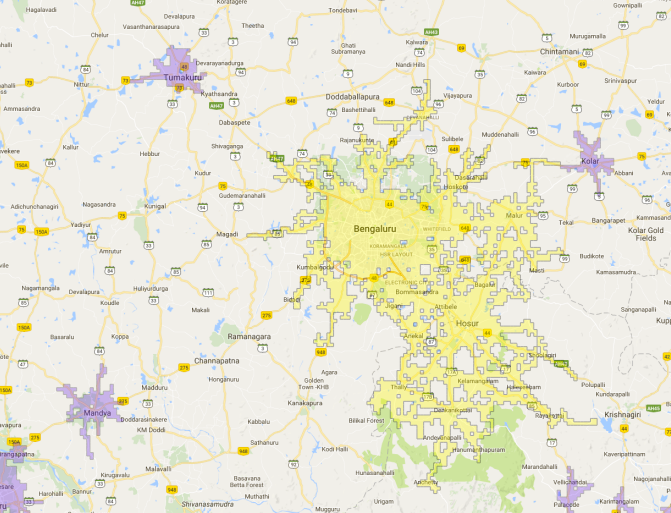
\includegraphics[width=\textwidth]{Bangalore}
  \caption{Geographic Definition of Bangalore}
   \label{fig:Bangalore}
\end{centering}
\end{figure}

\begin{longtable}{|p{0.5\textwidth}|p{0.30\textwidth}|}
\caption{Countries and their IPR scores \citep{Lesser2010}\label{long}}\\
 
 \hline\textbf{Country}&\textbf{IPR Score}\\\hline
 \endfirsthead
 
 \hline\textbf{Country}&\textbf{IPR Score}\\\hline
 \endhead
 
 \hline
 \endfoot
 
 \hline
 \endlastfoot
Afghanistan& \\\hline
Albania&4.7682 \\\hline
Algeria&2.7608 \\\hline
Angola&1.8734 \\\hline
Anguilla& \\\hline
Antigua and Barbuda& \\\hline
Argentina&5.4684 \\\hline
Armenia&4.4032 \\\hline
Aruba& \\\hline
Australia&11.1872 \\\hline
Austria&9.4024 \\\hline
Azerbaijan&3.1358 \\\hline
Bahamas& \\\hline
Bahrain&5.7736 \\\hline
Bangladesh&2.3664 \\\hline
Barbados& \\\hline
Belarus&3.2344 \\\hline
Belgium&9.6096 \\\hline
Belize& \\\hline
Benin& \\\hline
Bermuda& \\\hline
Bhutan&4.9300 \\\hline
Bolivia&4.2752 \\\hline
Bosnia and Herzegovina&2.9580 \\\hline
Botswana&6.2666 \\\hline
Brazil&5.2612 \\\hline
British Virgin Islands& \\\hline
Brunei Darussalam&5.4230 \\\hline
Bulgaria&5.3598 \\\hline
Burkina Faso&3.5496 \\\hline
Burma& \\\hline
Cambodia&1.9720 \\\hline
Cameroon&2.1692 \\\hline
Canada&11.1872 \\\hline
Cayman Islands& \\\hline
Central African Republic&1.9720 \\\hline
Chad&1.5776 \\\hline
Chile&9.2152 \\\hline
China&6.1586 \\\hline
Colombia&6.2572 \\\hline
Congo&1.8734 \\\hline
Cook Islands& \\\hline
Costa Rica&6.8388 \\\hline
Cote d'Ivoire&2.0706 \\\hline
Croatia&5.8528 \\\hline
Cuba& \\\hline
Cyprus&7.2526 \\\hline
Czech Republic&6.4444 \\\hline
Democratic Republic of the Congo&3.8260 \\\hline
Denmark&11.7788 \\\hline
Djibouti& \\\hline
Dominica& \\\hline
Dominican Republic& \\\hline
Ecuador&3.7822 \\\hline
Egypt&2.7608 \\\hline
El Salvador&3.3524 \\\hline
Equatorial Guinea& \\\hline
Estonia&9.1166 \\\hline
Ethiopia&2.6622 \\\hline
Fiji& \\\hline
Finland&11.3844 \\\hline
France&10.3984 \\\hline
French Guiana&10.3984 \\\hline
Gabon&2.8594 \\\hline
Gambia&2.8594 \\\hline
Georgia&4.9106 \\\hline
Germany&10.4970 \\\hline
Ghana&4.5904 \\\hline
Greece&5.4878 \\\hline
Greenland& \\\hline
Guadeloupe& \\\hline
Guam& \\\hline
Guatemala&3.3524 \\\hline
Guernsey& \\\hline
Guinea&1.7748 \\\hline
Guinea-Bissau& \\\hline
Guyana&2.5636 \\\hline
Haiti&1.7748 \\\hline
Honduras&3.2100 \\\hline
Hong Kong&8.0852 \\\hline
Hungary&7.6376 \\\hline
Iceland&10.1912 \\\hline
India&4.0974 \\\hline
Indonesia&4.5018 \\\hline
Iran (Islamic Republic of)&1.7748 \\\hline
Iraq&1.4790 \\\hline
Ireland&9.6290 \\\hline
Isle of Man& \\\hline
Israel&8.6236 \\\hline
Italy&6.8488 \\\hline
Jamaica&2.9580 \\\hline
Japan&10.2012 \\\hline
Jersey& \\\hline
Jordan&6.5430 \\\hline
Kazakhstan&2.6622 \\\hline
Kenya&3.7822 \\\hline
Korea, Democratic Republic of& \\\hline
Korea, Republic of&7.1640 \\\hline
Kuwait&4.0426 \\\hline
Kyrgyzstan&3.4864 \\\hline
Lao People's Democratic Republic&1.9720 \\\hline
Latvia&6.0500 \\\hline
Lebanon&2.4650 \\\hline
Lesotho& \\\hline
Liberia&3.0566 \\\hline
Libyan Arab Jamahiriya& \\\hline
Liechtenstein& \\\hline
Lithuania&7.4404 \\\hline
Luxembourg&8.8302 \\\hline
Macau& \\\hline
Madagascar&2.9580 \\\hline
Malawi&3.2538 \\\hline
Malaysia&5.1820 \\\hline
Mali&2.7608 \\\hline
Malta& \\\hline
Mauritania&2.4650 \\\hline
Mauritius&5.3244 \\\hline
Mexico&4.8668 \\\hline
Monaco& \\\hline
Mongolia&3.4072 \\\hline
Montenegro& \\\hline
Morocco&5.8628 \\\hline
Mozambique&2.4650 \\\hline
Namibia&4.4370 \\\hline
Nepal&2.2678 \\\hline
Netherlands Antilles&11.3844 \\\hline
Netherlands&11.3844 \\\hline
New Caledonia& \\\hline
New Zealand&11.8774 \\\hline
Nicaragua&5.0740 \\\hline
Niger&2.8594 \\\hline
Nigeria&3.2100 \\\hline
Northern Mariana Islands& \\\hline
Norway&10.1912 \\\hline
Oman&7.0360 \\\hline
Pakistan&4.1074 \\\hline
Palau& \\\hline
Palestine& \\\hline
Panama&5.2164 \\\hline
Papua New Guinea&2.0706 \\\hline
Paraguay&3.6836 \\\hline
Peru&5.3892 \\\hline
Philippines&4.1074 \\\hline
Poland&7.5390 \\\hline
Portugal&8.3278 \\\hline
Puerto Rico& \\\hline
Qatar&7.6470 \\\hline
Republic of Moldova&4.1218 \\\hline
Reunion& \\\hline
Romania&6.3558 \\\hline
Russia&4.0332 \\\hline
Saint Barthelemy& \\\hline
Saint Kitts and Nevis& \\\hline
Saint Lucia& \\\hline
Saint Pierre and Miquelon& \\\hline
San Marino& \\\hline
Saudi Arabia&4.2398 \\\hline
Senegal&2.9580 \\\hline
Serbia&4.4470 \\\hline
Seychelles& \\\hline
Sierra Leone&2.1692 \\\hline
Singapore&11.6802 \\\hline
Slovakia&7.0460 \\\hline
Slovenia&8.3716 \\\hline
Solomon Islands& \\\hline
South Africa&7.2432 \\\hline
Spain&8.6236 \\\hline
Sri Lanka&3.0566 \\\hline
Sudan&1.4790 \\\hline
Suriname&3.6482 \\\hline
Svalbard& \\\hline
Swaziland&4.2946 \\\hline
Sweden&11.6802 \\\hline
Switzerland&11.4830 \\\hline
Syrian Arab Republic&3.5596 \\\hline
Taiwan&7.2626 \\\hline
Tajikistan&1.9720 \\\hline
Thailand&4.0974 \\\hline
The former Yugoslav Republic of Macedonia& \\\hline
Togo&2.7608 \\\hline
Trinidad and Tobago&5.1626 \\\hline
Tunisia&5.8528 \\\hline
Turkey&6.9474 \\\hline
Turkmenistan& \\\hline
Turks and Caicos Islands& \\\hline
Uganda&2.4650 \\\hline
Ukraine&3.7822 \\\hline
United Arab Emirates&6.4090 \\\hline
United Kingdom&10.2012 \\\hline
United Republic of Tanzania&2.5636 \\\hline
United States Virgin Islands&10.0040 \\\hline
United States&10.0040 \\\hline
Uruguay&8.2192 \\\hline
Uzbekistan&3.6388 \\\hline
Venezuela&3.6144 \\\hline
Vietnam&4.2752 \\\hline
Yemen&2.0706 \\\hline
Zambia&2.9580 \\\hline
Zimbabwe&2.9142 \\\hline
\end{longtable}



\end{document}
